
In the parametric analysis of \Cyder performance, it was shown that sorption
sensitivity behavior closely matched that of the \gls{GDSM} sensitivity
behaviors. Specifically, in Figure \ref{fig:kd_result}, increasing the retardation
coefficient results in a smooth but dramatic turnover.

\begin{figure}[ht]
\centering
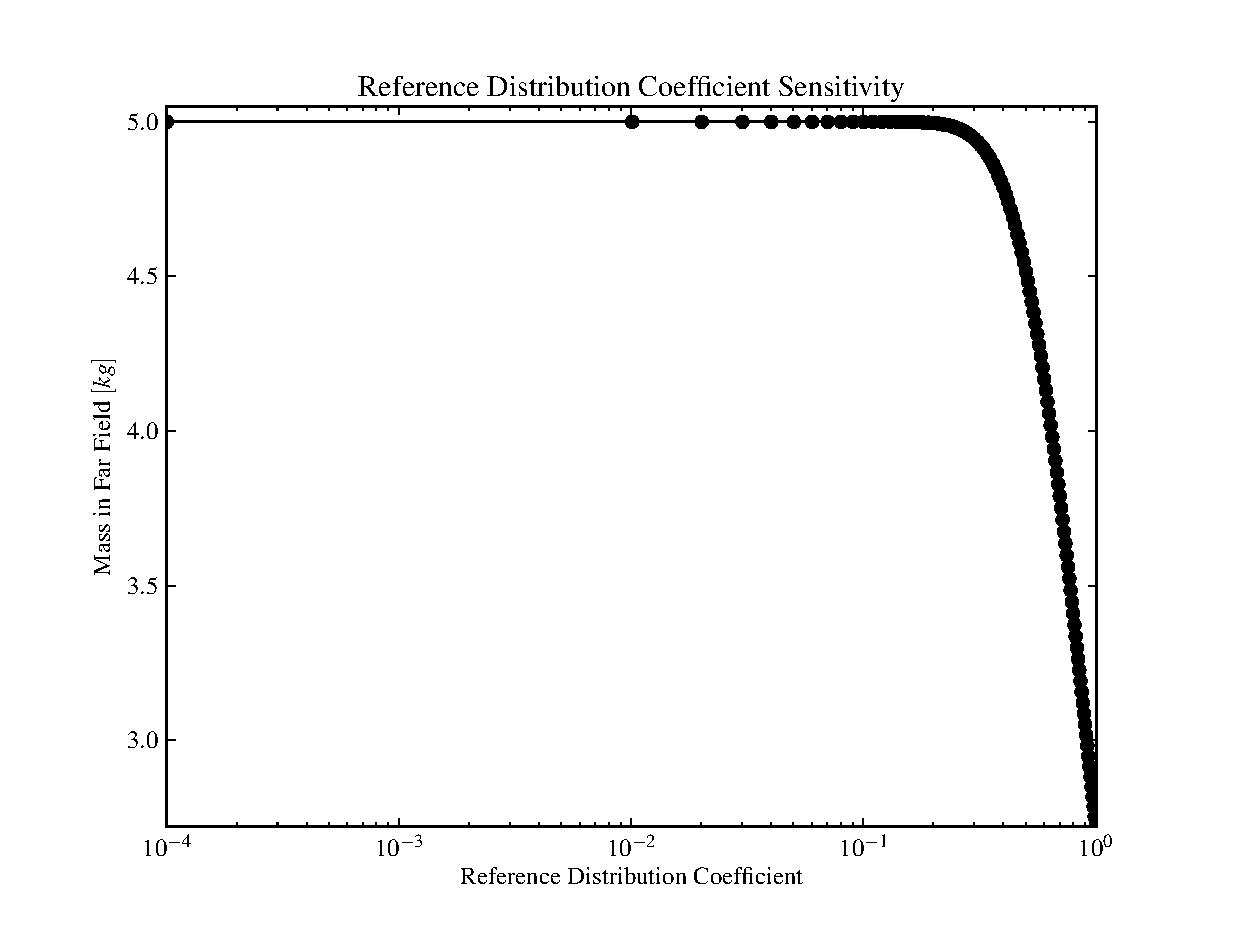
\includegraphics[width=0.7\linewidth]{./results/images/kd.eps}
\caption[$K_d$ sensitivity in the Mixed Cell Model]{$K_d$ sensitivity in the
\Cyder tool for an arbitrary isotope assigned a variable $K_d$ coefficient.}
\label{fig:kd_result}
\end{figure}
